%% Mechanical Systems and Signal Processing -- submission manuscript
%% Elsevier elsarticle class, numbered reference style (elsarticle-num).
%%
%% NOT COMPILED: no TeX toolchain was available in the environment this was
%% written in. Compile with
%%     latexmk -pdf manuscript.tex
%% before submitting, and check the items listed in README.md.

\documentclass[preprint,12pt]{elsarticle}

\usepackage{amsmath}
\usepackage{amssymb}
\usepackage{booktabs}
\usepackage{graphicx}
\usepackage{url}
\usepackage[T1]{fontenc}
\usepackage[utf8]{inputenc}

\journal{Mechanical Systems and Signal Processing}

\begin{document}

\begin{frontmatter}

\title{Goodness-of-fit is not validity: residual camera motion in
model-based operating deflection shapes from video}

%% TODO before submission: complete author list, affiliations and ORCIDs.
\author[keti]{J.-H. Chae\corref{cor1}}
\ead{jhchae@keti.re.kr}
\cortext[cor1]{Corresponding author.}

\affiliation[keti]{organization={Korea Electronics Technology Institute},
            country={Republic of Korea}}

\begin{highlights}
\item Camera ego-motion lies inside the span of parametric ODS models
\item Model fit $R^2$ is anti-correlated with true shape accuracy, $r=-0.162$
\item 2 px of uncompensated scene motion halves video ODS shape fidelity
\item Affine compensation on static regions holds MAC $\ge$ 0.92 to 4 px
\item Four sensor-free consistency checks replace goodness-of-fit
\end{highlights}

\begin{abstract}
Video-based operating deflection shape (ODS) measurement increasingly fits
the measured full-field motion to a parametric structural model, both to
regularise noisy optical flow and to obtain a three-dimensional shape from a
single view. Where no reference accelerometer is available, the
goodness-of-fit of that model is the natural self-check, and is often the
only quantitative validity figure reported. This paper shows that the check
is not merely weak but inverted. Residual camera ego-motion produces an
affine displacement field, and we prove that this field lies inside the span
of the structural model: for a cylinder-station model, camera translation
and image shear are reproduced with $R^2 = 1.0000$ exactly and camera roll
converges to unity as the axial station binning is refined, while a genuine
cantilever deflection fits no better. In a controlled experiment with a
known injected deflection shape and a known injected camera roll, the
correlation between model $R^2$ and the modal assurance criterion against
the injected shape is $r = -0.162$ over 15 runs; a run whose recovered shape
is destroyed (MAC 0.060) reports $R^2 = 0.752$, whereas a run whose shape is
nearly correct (MAC 0.920) reports $R^2 = 0.458$. Approximately 2 px of
uncompensated scene motion halves shape fidelity and 4 px destroys it, while
an affine compensation fitted on static reference regions maintains
MAC $\ge 0.92$ to 4 px. Four internal-consistency checks are proposed in
place of fit quality, and applying them retracts a previously published
deflection shape.
\end{abstract}

\begin{keyword}
operating deflection shape \sep video vibration measurement \sep
camera ego-motion \sep model identifiability \sep optical flow \sep
modal assurance criterion
\end{keyword}

\end{frontmatter}

%% ------------------------------------------------------------------
\section{Introduction}
\label{sec:intro}

A camera pointed at a running machine measures every pixel at once, which is
what makes video attractive for ODS work: no accelerometer mass loading, no
cabling, and hundreds of effective measurement points. Two families of
technique dominate, phase-based motion magnification for visualisation and
optical flow for quantitative displacement extraction.

Both produce a two-dimensional field. Turning that field into an operating
deflection shape on a structure usually means fitting it to something: a set
of axial stations, a beam model, a parametric geometry. The fit does real
work. It denoises, it separates axial from transverse response, and, for a
single camera, it is the only route to a three-dimensional shape, since one
view cannot resolve motion along the optical axis.

Having fitted a model, the natural question is whether the fit is any good,
and the natural answer is a goodness-of-fit statistic: $R^2$, residual norm,
or explained variance. In the absence of a reference sensor this is often
the only quantitative claim of validity a video ODS result carries.

This paper argues that the statistic answers a different question from the
one being asked, and answers it in a way that is actively misleading. The
argument has three parts: an identifiability analysis
(Section~\ref{sec:ident}), a controlled experiment with ground truth
(Section~\ref{sec:controlled}), and a field case in which following the
statistic produced a confidently wrong result that we retract
(Section~\ref{sec:field}).

The contributions are as follows.
\begin{enumerate}
\item A proof, with numerical confirmation, that the affine field produced
  by camera ego-motion lies inside the span of a standard cylinder-station
  ODS model, exactly so for translation and image shear
  (Section~\ref{sec:ident}).
\item A controlled experiment quantifying the resulting inversion: $R^2$ is
  uncorrelated to anti-correlated with true shape fidelity
  ($r = -0.162$), and approximately 2 px of uncompensated scene motion
  halves the modal assurance criterion (Section~\ref{sec:controlled}).
\item A field case demonstrating the failure on real data, and the
  retraction of a previously published deflection shape
  (Section~\ref{sec:field}).
\item Four sensor-free internal-consistency checks that do have
  discriminating power, with the discriminating one identified
  (Section~\ref{sec:checks}).
\end{enumerate}

%% ------------------------------------------------------------------
\section{Related work}
\label{sec:related}

\paragraph{ODS from video}
Extraction of operating deflection shapes directly from optical flow, with
automatic masking and frame-wise fusion, is established \cite{machynia2021}.
Phase-based Eulerian motion magnification has been used to visualise ODS and
to identify modal parameters of civil structures
\cite{chen2015,chen2017}, building on the phase-based motion processing of
\cite{wadhwa2013}. Commercial systems productise the workflow.

\paragraph{Three-dimensional ODS from cameras}
A single two-dimensional view cannot resolve motion along the optical axis.
Frequency-domain triangulation \cite{gorjup2019} and multiview spectral
optical flow imaging \cite{gorjup2021} recover full-field three-dimensional
ODS using multiple views precisely for this reason. Fitting a single view to
a parametric three-dimensional geometry, as studied here, is the cheap
alternative, and, as Section~\ref{sec:ident} shows, the one that opens the
identifiability hole.

\paragraph{Camera motion compensation}
Compensating camera ego-motion using static reference regions outside the
structure, by affine or homography transforms estimated on reference
templates, is standard practice in vision-based structural health monitoring
\cite{chen2017}. Section~\ref{sec:field} measures it dominating outright:
83\% of the band energy on our field clip, moving the static background more
than the machine. Our contribution is not the compensation itself but the
demonstration that its \emph{absence} is rewarded by the fit statistic, so a
pipeline missing it receives no warning and in fact receives encouragement.

\paragraph{Goodness-of-fit critiques}
That $R^2$ rewards added parameters and does not establish model correctness
is elementary. What is specific here is the structural coincidence: the
nuisance field and the signal model are not merely both flexible, they
overlap exactly, which makes the statistic not just uninformative but
reversed.

%% ------------------------------------------------------------------
\section{Method under study}
\label{sec:method}

We study a pipeline representative of the class. Motion vectors are obtained
by dense Farneb\"ack optical flow measured frame-to-reference. A
Hann-windowed discrete Fourier transform per point gives complex amplitude
and phase at the analysis line. Points are binned into axial stations along
the machine axis, and per station $j$ a complex linear least-squares fit
separates
\begin{align}
u(\theta) &= dX_j + \varphi_j\,(z/R), \label{eq:u}\\
v(\theta) &= dZ_j + \left[a_{2,j}\cos 2\theta
             + b_{2,j}\sin 2\theta\right]\cos\theta, \label{eq:v}
\end{align}
where $u$ and $v$ are image-horizontal and image-vertical displacement,
$\theta$ is the circumferential angle of the point on the visible face,
$dX_j$ is axial translation, $\varphi_j$ is section rocking, $dZ_j$ is
transverse translation, and $a_2$, $b_2$ are the $n = 2$ ovalization
coefficients projected onto the visible face. Out-of-plane translation is
unobservable from one view and is set to zero. The station fits are expanded
onto the nodes of a parametric cylinder geometry to give a
three-dimensional shape.

The reported fit statistic is
\begin{equation}
R^2 = 1 - \frac{\sum \lvert d_{\mathrm{meas}}
                 - d_{\mathrm{pred}}\rvert^2}
                {\sum \lvert d_{\mathrm{meas}}
                 - \bar{d}_{\mathrm{meas}}\rvert^2},
\label{eq:r2}
\end{equation}
taken over all measurement points, with $d = (u, v)$ complex.

%% ------------------------------------------------------------------
\section{The structural model spans the camera field}
\label{sec:ident}

\subsection{Analysis}
\label{sec:ident-analysis}

Let the camera undergo a small rigid motion between the reference frame and
frame $t$. To first order the induced image displacement of a sufficiently
distant, sufficiently planar scene is affine,
\begin{equation}
\mathbf{d}(\mathbf{p}) = \mathbf{A}\mathbf{p} + \mathbf{t},
\qquad
\mathbf{A} = \begin{bmatrix} a_{11} & a_{12}\\
                             a_{21} & a_{22}\end{bmatrix},
\label{eq:affine}
\end{equation}
where camera translation contributes $\mathbf{t}$, roll about the optical
axis contributes the antisymmetric part of $\mathbf{A}$, pan and tilt
contribute to first order further translation, and dolly contributes the
isotropic part.

Write this per axial station. Within station $j$ the axial coordinate is
$x = x_j$, constant, while the transverse coordinate $z$ varies across the
ring. Then
\begin{align}
u &= (t_u + a_{11}x_j) + a_{12}z, \label{eq:cam-u}\\
v &= (t_v + a_{21}x_j) + a_{22}z. \label{eq:cam-v}
\end{align}

Compare with Eqs.~\eqref{eq:u}--\eqref{eq:v}. The $u$ row is spanned
\emph{exactly}: the constant term is $dX_j$ and the term linear in $z$ is
precisely the rocking degree of freedom $\varphi_j (z/R)$. There is no
residual, for any camera motion.

The $v$ row is spanned in its constant term by $dZ_j$. Its term linear in
$z$ has no dedicated degree of freedom and must be supplied by the
ovalization basis. With $z = R\sin\theta$,
\begin{equation}
\sin 2\theta\cos\theta
  = \tfrac{1}{2}\left(\sin\theta + \sin 3\theta\right),
\label{eq:drag}
\end{equation}
so the $b_2$ coefficient buys the required $\sin\theta$ only in fixed
one-to-one company with a $\sin 3\theta$ the field does not contain. The
entire residual of an affine camera field under this model is that unwanted
$\sin 3\theta$, and any camera motion whose $v$ does not vary with $z$
(translation, roll, $\partial v/\partial x$ shear) leaves no residual at
all.

\subsection{Numerical confirmation}
\label{sec:ident-numeric}

We fed the fitter camera fields containing zero machine deflection and
recorded the $R^2$ returned. Table~\ref{tab:ident} and
Fig.~\ref{fig:ident}(a) give the result.

\begin{table}[htbp]
\centering
\caption{Model fit $R^2$ for pure camera fields, with no machine deflection
present. The final row is a genuine deflection shape, for contrast.}
\label{tab:ident}
\begin{tabular}{lrr}
\toprule
Camera field & $R^2$ (with rocking) & $R^2$ (no rocking)\\
\midrule
Translation                     & 1.0000 & 1.0000\\
Roll                            & 0.9843 & 0.5593\\
Shear $\partial u/\partial z$   & 1.0000 & 0.0000\\
Shear $\partial v/\partial x$   & 0.9726 & 0.9726\\
Zoom                            & 0.8109 & 0.8109\\
General affine                  & 0.9771 & 0.4654\\
\midrule
\emph{True cantilever bending} $v \sim x^2$ & \emph{0.9774} & ---\\
\bottomrule
\end{tabular}
\end{table}

\begin{figure}[htbp]
\centering
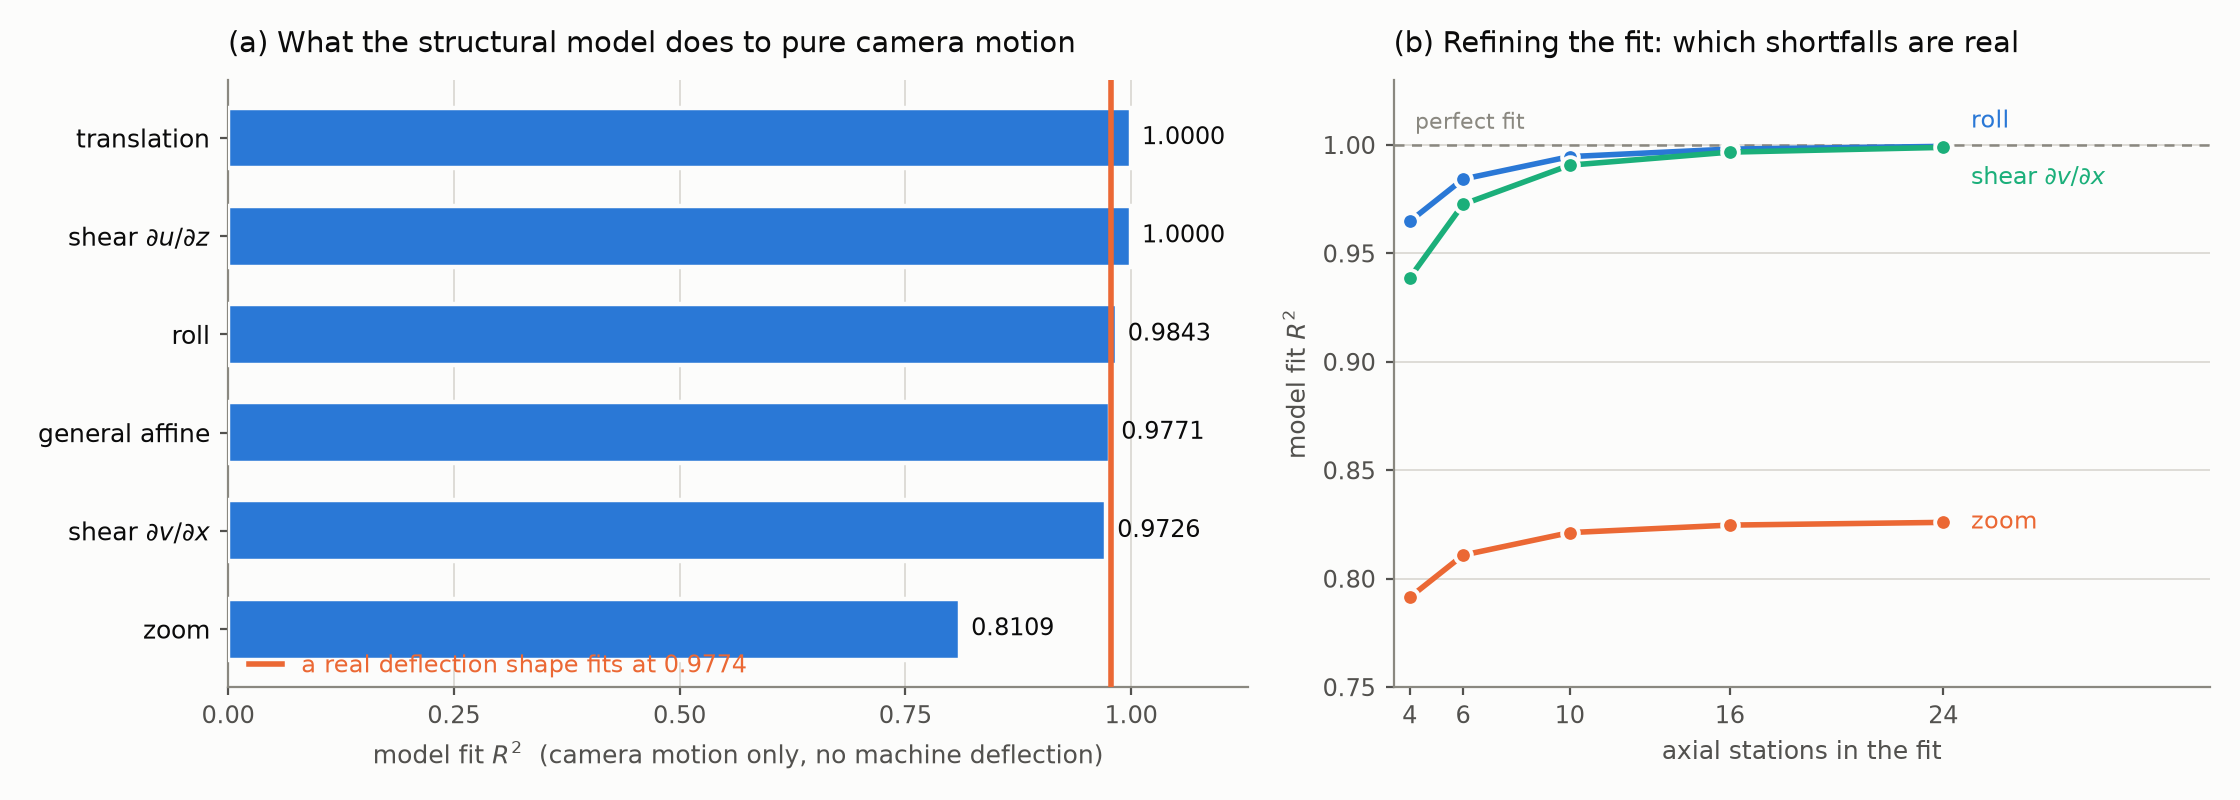
\includegraphics[width=\textwidth]{figs/fig1_identifiability.png}
\caption{(a) Model fit $R^2$ for pure camera fields with no machine
deflection present; the vertical line marks where a genuine cantilever
deflection fits. Two camera fields are fitted perfectly, and three fit
better than the real deflection does. (b) Refining the axial station count
separates the two kinds of shortfall: roll and $\partial v/\partial x$
converge to unity, so their residual was only binning width, whereas zoom
plateaus at the $\sin 3\theta$ drag predicted by Eq.~\eqref{eq:drag}.}
\label{fig:ident}
\end{figure}

Three things follow.

\paragraph{The exact cases are exact}
Translation and $\partial u/\partial z$ shear return $R^2 = 1.0000$. A
pipeline reporting a perfect fit may be looking at a scene with no
structural motion in it whatsoever.

\paragraph{The near-exact cases are limited only by station binning}
Roll and $\partial v/\partial x$ shear put a term linear in $x$ into $v$;
since a ring spans a range of $x$, the station fit absorbs it only to
binning resolution. Refining the stations confirms the prediction
(Table~\ref{tab:stations}, Fig.~\ref{fig:ident}(b)). Roll and
$\partial v/\partial x$ converge to unity, so their shortfall was never
structural. Zoom plateaus near 0.83, and that plateau is exactly the
$\sin 3\theta$ drag of Eq.~\eqref{eq:drag}, the only part of an affine field
the model genuinely cannot absorb.

\begin{table}[htbp]
\centering
\caption{Model fit $R^2$ against the number of axial stations in the fit.}
\label{tab:stations}
\begin{tabular}{lrrrrr}
\toprule
Camera field & 4 & 6 & 10 & 16 & 24\\
\midrule
Roll                          & 0.9647 & 0.9843 & 0.9946 & 0.9981 & 0.9994\\
Shear $\partial v/\partial x$ & 0.9387 & 0.9726 & 0.9907 & 0.9967 & 0.9989\\
Zoom                          & 0.7914 & 0.8109 & 0.8213 & 0.8247 & 0.8260\\
\bottomrule
\end{tabular}
\end{table}

\paragraph{A real deflection shape fits no better than camera motion}
The cantilever bending case returns $R^2 = 0.9774$, lower than translation
(1.0000), lower than $\partial u/\partial z$ shear (1.0000), lower than roll
at any station count above six, and indistinguishable from the general
affine camera field (0.9771). This is the crux: $R^2$ has no discriminating
power between the signal and the nuisance, because the nuisance is inside
the model space.

\subsection{The rocking degree of freedom is the mechanism}
\label{sec:rocking}

Table~\ref{tab:ident} also prices the modelling choice. Adding the section
rocking degree of freedom $\varphi_j$ raises the fit of
$\partial u/\partial z$ camera shear from 0.0000 to 1.0000, and of general
affine camera motion from 0.4654 to 0.9771. Rocking is physically well
motivated, since machines do rock on their mounts, but it is also precisely
the shape a rolling camera writes into $u$. A degree of freedom added to
capture real physics silently doubled as the absorber for the dominant
artefact.

%% ------------------------------------------------------------------
\section{Controlled experiment}
\label{sec:controlled}

\subsection{Design}

The analysis says the model can absorb camera motion. The operational
question is how much shape error that buys at realistic amplitudes. We built
a harness with ground truth:
\begin{enumerate}
\item take a real still frame of the machine, so that texture, contrast and
  flow behaviour are realistic;
\item warp it by a \emph{known} deflection shape, cantilever-like,
  $s(x) = x^2(3 - 2x)$, with 2.0 px peak at the free end, confined to the
  machine region;
\item add a \emph{known} whole-scene camera roll at the same frequency,
  swept in amplitude;
\item run the pipeline and score the recovered station profile against the
  injected shape by the modal assurance criterion (MAC), and the recovered
  peak against the injected peak as an amplitude gain.
\end{enumerate}
MAC and gain cannot be inflated by absorbing camera motion, because the
truth is known independently of the fit.

Two design points matter. First, the injected scene motion is a \emph{roll},
not a horizontal shear. An earlier version of this experiment injected
horizontal shear while the machine deflected vertically; the pipeline scored
MAC $\ge 0.98$ at every amplitude with no compensation at all, because the
disturbance and the measurand never overlapped. It passed for the wrong
reason. A roll has a vertical component that competes directly with the
transverse deflection being measured. Second, the amplitude sweep is capped
so that whole-frame camera displacement stays inside the optical-flow
capture range; beyond that the breakdown measured is Farneb\"ack's, not the
method's.

\subsection{Results}

Table~\ref{tab:mac} and Fig.~\ref{fig:controlled}(a) give shape fidelity
against injected camera motion. Uncompensated scene motion of approximately
2 px halves shape fidelity, from 0.982 to 0.611, and approximately 4 px
destroys it, to 0.268. Affine compensation fitted on static reference
regions holds MAC $\ge 0.92$ out to approximately 4 px. Mean-only
compensation, which subtracts the average displacement of a reference region
and so cancels an offset while leaving the gradient intact, recovers only
part of the loss. Beyond approximately 8 px the affine fit itself degrades,
as the reference regions no longer constrain a field that large.

\begin{table}[htbp]
\centering
\caption{MAC against the injected shape, by scene-motion compensation mode.}
\label{tab:mac}
\begin{tabular}{lrrr}
\toprule
Scene motion & None & Mean only & Affine\\
\midrule
0.00 px & 0.982 & 0.982 & 0.982\\
0.99 px & 0.860 & 0.939 & 0.975\\
1.98 px & 0.611 & 0.831 & 0.965\\
3.95 px & 0.268 & 0.741 & 0.920\\
7.90 px & 0.060 & 0.717 & 0.640\\
\bottomrule
\end{tabular}
\end{table}

\begin{figure}[htbp]
\centering
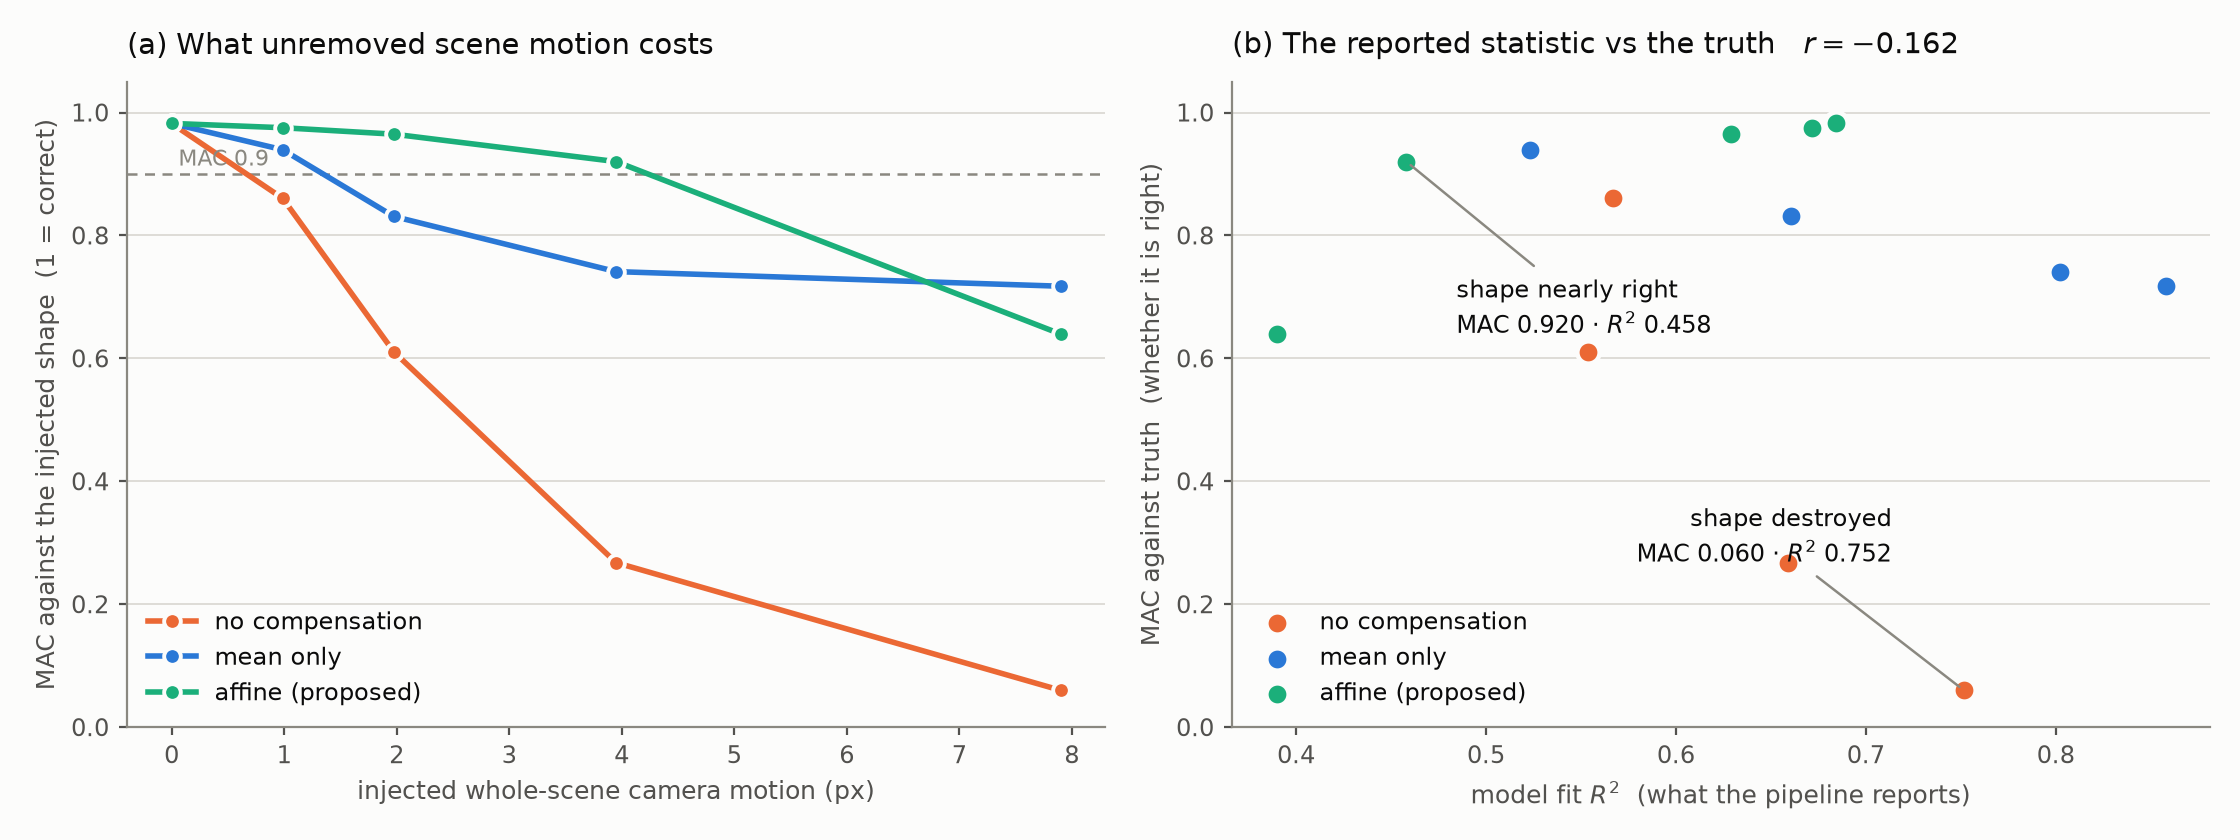
\includegraphics[width=\textwidth]{figs/fig2_controlled.png}
\caption{(a) Shape fidelity against injected camera motion for the three
compensation modes. (b) The same 15 runs plotted as reported statistic
against actual correctness; a useful self-check would trend up and to the
right, and this one does not.}
\label{fig:controlled}
\end{figure}

The correlation between model $R^2$ and true MAC over all 15 runs is
$r = -0.162$: not weakly positive, but slightly negative
(Fig.~\ref{fig:controlled}(b)). The sharpest pair is given in
Table~\ref{tab:pair}. The run whose recovered shape is destroyed reports a
fit statistic 1.6 times better than the run whose shape is nearly correct.

\begin{table}[htbp]
\centering
\caption{The sharpest pair of runs: the better fit statistic belongs to the
worse answer.}
\label{tab:pair}
\begin{tabular}{lrr}
\toprule
Run & MAC (truth) & $R^2$ (reported)\\
\midrule
7.90 px, no compensation     & 0.060 & 0.752\\
3.95 px, affine compensation & 0.920 & 0.458\\
\bottomrule
\end{tabular}
\end{table}

\subsection{Two by-products}

\paragraph{Amplitude gain is a usable warning without ground truth}
Recovered peak over true peak sits at 0.5--0.6 in every run where the shape
is essentially correct, and climbs past 1.0, to 1.75 and 1.36, only in runs
where the shape has collapsed. Scene motion inflates reported deflection; it
never shrinks it. A video ODS reporting larger amplitudes than expected
should be suspected, not celebrated.

\paragraph{The pipeline under-reports amplitude even when correct}
With the camera perfectly still and MAC 0.982, the gain is 0.58, an
under-report of approximately 43\%. Two mechanisms contribute: per-station
least squares averages over points whose true deflection varies within the
station, and Farneb\"ack smooths sub-pixel motion. Absolute amplitudes from
this class of pipeline require calibration before they are quoted in
engineering units.

%% ------------------------------------------------------------------
\section{Field case, and a retraction}
\label{sec:field}

\subsection{The clip}

A 30 frames per second handheld-class recording of a small motor rig on an
optical breadboard, excited at 6 Hz, with the motor casing, a gearbox, a
shaft and a belt pulley in view along with a wall, a floor and an aluminium
extrusion frame that are not attached to the rig.

A previously published run of our own pipeline on this clip produced a
three-dimensional deflection shape with a drive-end to free-end amplitude
growth of 0.85 px to 2.4 px, described as vertical bending, and reported a
model fit of $R^2 = 0.99$.

\subsection{What the clip actually contains}

Fitting a complex affine field to the whole frame at the analysis line
explains 83\% of the 6 Hz band energy. Measured region by region on the raw
field, the static background moves \emph{more} than the machine
(Table~\ref{tab:regions}, Fig.~\ref{fig:field}(a)). The field is a shear,
$\partial u/\partial y \approx 13$ px per 100 px, which is a camera that
rocks rather than one that shifts, and so exactly the case
Section~\ref{sec:ident} shows the model absorbs through its rocking degree
of freedom.

\begin{table}[htbp]
\centering
\caption{6 Hz amplitude by region on the motor clip, raw field and after
affine compensation, with narrowband signal-to-noise ratio of the
compensated residual. Regions marked static are not attached to the rig.}
\label{tab:regions}
\begin{tabular}{lrrr}
\toprule
Region & Raw (px) & Compensated (px) & SNR\\
\midrule
Motor casing        & 1.68 & 0.298 & 407\\
Gearbox / shaft     & 1.26 & 0.539 & 1986\\
Belt pulley         & 0.63 & 0.280 & 301\\
Wall (static)       & 2.03 & 0.655 & 1440\\
Floor (static)      & ---  & 0.602 & 1438\\
Extrusion (static)  & 2.15 & ---   & ---\\
\bottomrule
\end{tabular}
\end{table}

\begin{figure}[htbp]
\centering
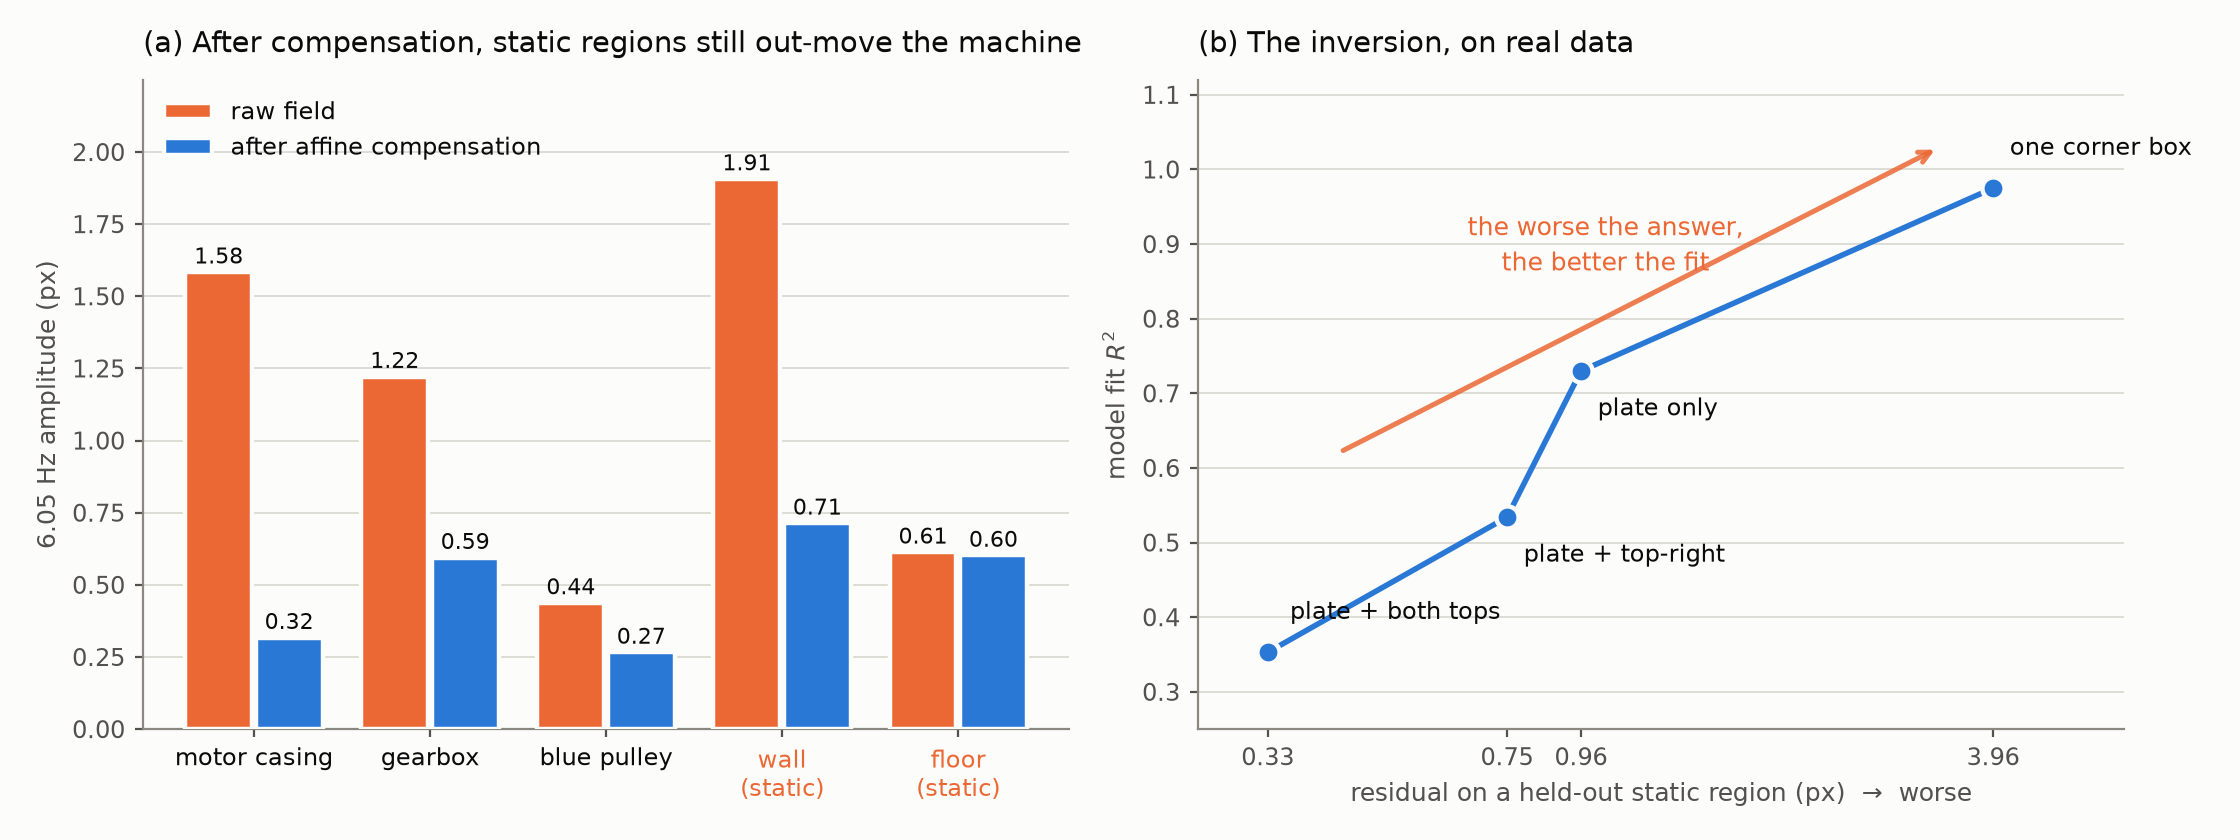
\includegraphics[width=\textwidth]{figs/fig3_field.png}
\caption{(a) 6 Hz amplitude by region on the motor clip, before and after
affine compensation. In the raw field the wall out-moves the motor casing;
the floor does not, being nearer the quiet end of the camera gradient. After
compensation both static regions retain more than the casing, which is the
comparison that matters, since it is the residual the restoration actually
works from. (b) Varying only the quality of the compensation traces out the
inversion: the fit statistic climbs as the answer gets worse.}
\label{fig:field}
\end{figure}

After affine compensation fitted on three static reference boxes straddling
the frame, the static wall and floor retain \emph{more} coherent 6 Hz motion
than the motor casing does. Whatever the residual is, whether parallax
across depth, rolling shutter, or a camera field that is not exactly affine,
it is not separable from the machine's own deformation at this amplitude.
This clip contains no recoverable machine ODS at 6 Hz.

\subsection{The inversion on real data}

Varying only the quality of the scene-motion removal traces out
Table~\ref{tab:inversion} and Fig.~\ref{fig:field}(b). The fit statistic is
monotonically anti-correlated with the quality of the compensation. The same
holds for the assumed machine axis: uncompensated, $R^2$ climbs from 0.833
at the machine's visible axis ($-15^\circ$) to 0.943 at $+51^\circ$, that
is, the fit improves as the model is pointed \emph{away} from the machine,
because a rotated frame lets it absorb the gradient more efficiently.

\begin{table}[htbp]
\centering
\caption{Fit statistic against actual answer quality on the motor clip.}
\label{tab:inversion}
\begin{tabular}{lrrr}
\toprule
Scene-motion removal & Held-out static residual (px)
                     & Casing amplitude (px) & $R^2$\\
\midrule
One corner box (poor fit) & 3.960 & 2.617 & 0.975\\
Plate only                & 0.965 & 0.718 & 0.730\\
Plate $+$ top-right       & 0.749 & 0.487 & 0.534\\
Plate $+$ both tops       & 0.330 & 0.288 & 0.353\\
\bottomrule
\end{tabular}
\end{table}

\subsection{Retraction}

The published result is withdrawn. The 0.85 px to 2.4 px profile was the
camera's gradient, not the machine's deflection, and the 2.4 px end was
further inflated by drift in accumulated frame-to-frame optical flow
(0.616 px median, 4.442 px at the 90th percentile over 120 frames, against a
signal of approximately 2.5 px). Three ordinary defects contributed. The
clip is stored rotated by $90^\circ$ and was analysed sideways; the machine
axis was set to $+15.3^\circ$ when the data put it at $-76.2^\circ$ in that
frame, swapping axial and transverse; and the flow was accumulated rather
than measured against a reference. None of them is the reason the result
looked convincing. It looked convincing because $R^2 = 0.99$, and
$R^2 = 0.99$ is what Section~\ref{sec:ident} predicts for a scene dominated
by camera roll.

%% ------------------------------------------------------------------
\section{What to report instead}
\label{sec:checks}

No single statistic replaces a reference sensor. Table~\ref{tab:checks}
lists four internal-consistency checks, each asking a question that a
genuine deflection answers differently from residual camera motion.

\begin{table}[htbp]
\centering
\caption{Sensor-free internal-consistency checks.}
\label{tab:checks}
\begin{tabular}{lll}
\toprule
Check & Rules out & Requires\\
\midrule
Static region & Scene motion, directly & One clip\\
Split-half    & Non-stationarity, flow noise & One clip\\
Repeat        & Camera artefacts, near-conclusively
              & \emph{Two recordings}\\
Order lock    & Anything ignorant of shaft speed
              & One clip $+$ known rpm\\
\bottomrule
\end{tabular}
\end{table}

\paragraph{Static region}
Hold a region that cannot be moving \emph{out} of the compensation reference
set, and measure what survives there at the analysis line relative to the
structure. On the clip of Section~\ref{sec:field} this returns machine
0.295 px against static 0.714 px, a ratio of $0.41\times$, and the check
fires. We propose a ratio of at least 2 as a necessary precondition for any
downstream claim.

Two implementation points, both learned by pointing the check at the field
clip as a control. First, the ratio must be measured \emph{after} the same
compensation the restoration applies; measured on the raw field, on a clip
whose dominant field is a gradient, it compares the gradient's hot end to
its cold end and flatters any structure that happens to sit at the hot end.
On the field clip the uncorrected form reported $2.00\times$ and usable,
where the corrected form reports $0.44\times$ and reject. Second, regions
chosen automatically from band power pick the two ends of that same
gradient, so automatically chosen regions must return \emph{unconfirmed}
rather than a verdict.

\paragraph{Split-half}
Restore from the first and second halves of one recording independently and
correlate. This is necessary but \emph{not} sufficient, and the field clip
is the counterexample: it scores MAC 1.000. Both halves share the same
camera, so a steady camera-driven shape reproduces perfectly. A check that
cannot distinguish a steady camera from a steady machine should never be
reported alone.

\paragraph{Repeat}
Restore from two \emph{separate recordings} of the same machine state and
correlate. Camera motion is uncorrelated between recordings, whether a
different tripod settling or a different phase of building sway, while the
machine's deflection shape is not. This is the check that justifies changing
how data is captured, and the one we could not run
(Section~\ref{sec:limits}).

\paragraph{Order lock}
For rotating machinery, response concentrates at integer orders of running
speed. Given the shaft speed, report the deviation of the dominant peak from
first order and the order-locked share of band energy. Building sway, hand
shake and rolling shutter do not know the shaft speed. This is nearly free
and should be standard whenever the speed is known.

%% ------------------------------------------------------------------
\section{Limitations}
\label{sec:limits}

\paragraph{No reference sensor}
Every claim about the real clip rests on video alone. Two accelerometers are
visible in the frame; their signals were not available. This is the single
largest gap and the first thing to close.

\paragraph{The field case is negative}
Section~\ref{sec:field} demonstrates the failure mode but is not a
demonstration that the restoration works when conditions are good. A
tripod-mounted, higher-amplitude, global-shutter recording would supply the
positive case. We screened all available footage against the checks of
Section~\ref{sec:checks} and none passed: every clip failed on the
scene-motion ratio, on reproduction within its own recording, or on length.

\paragraph{The repeat check is unexercised}
It is the strongest of the four and has not been run on real data, because
it needs two independent recordings of one machine state and none were
available.

\paragraph{One geometry}
The analysis of Section~\ref{sec:ident} is worked for the cylinder-station
model. The argument generalises to any low-order structural basis containing
per-station translation and a rotation-like degree of freedom, which is most
of them, but the exact $R^2$ values are model-specific.

\paragraph{First-order affine}
Real camera motion over a scene with depth is not exactly affine. Parallax
is precisely what we suspect remains in the static-region residual of
Table~\ref{tab:regions}, and a compensation model richer than affine may
recover more.

%% ------------------------------------------------------------------
\section{Conclusion}
\label{sec:conclusion}

The goodness-of-fit of a structural model, computed on the same field it was
fitted to, cannot validate a video-derived operating deflection shape,
because the dominant nuisance, residual camera ego-motion, lies inside the
model's span. For the cylinder-station model studied here it lies inside
exactly for camera translation and image shear, and to within station
binning for camera roll. A real deflection shape fits no better than a pure
camera field, and in our controlled experiment the fit statistic is slightly
anti-correlated, $r = -0.162$, with true shape fidelity.

The practical consequences are concrete. Compensate scene motion with an
affine field fitted on static reference regions rather than a mean offset;
hold a static region out of that fit and report what survives there; treat
split-half reproduction as necessary rather than sufficient; record twice
and report the cross-recording MAC; and, for rotating machinery, report
order lock against the known shaft speed. Report amplitude gain as a warning
flag, and calibrate before quoting absolute deflections.

We applied these to our own prior result and withdrew it. The same test is
worth applying to any video ODS whose only quantitative claim of validity is
that the model fitted well.

%% ------------------------------------------------------------------
\section*{CRediT authorship contribution statement}

%% TODO before submission: complete for all authors.
\textbf{J.-H. Chae:} Conceptualization, Methodology, Software, Validation,
Formal analysis, Investigation, Data curation, Writing -- original draft,
Writing -- review \& editing, Visualization.

\section*{Declaration of competing interest}

The authors declare that they have no known competing financial interests or
personal relationships that could have appeared to influence the work
reported in this paper.

\section*{Data availability}

%% TODO before submission: replace with the archived DOI (e.g. Zenodo).
The analysis code and the derived data behind every figure and table are
available at \url{https://github.com/dnfl5345/VibraStudio}. The field video
is not redistributable.

\section*{Acknowledgements}

%% TODO before submission: funding sources, or state that none were received.

%% ------------------------------------------------------------------
\bibliographystyle{elsarticle-num}
\bibliography{references}

\end{document}
